\documentclass[style=sailor,size=12pt]{powerdot}
\usepackage{epic,array,ecltree,url,calrsfs}
\usepackage[nointegrals]{wasysym}
\usepackage{listings}
\usepackage{epsfig}
\usepackage{amsmath}
\usepackage{amsfonts}
\usepackage{amssymb}
\usepackage{amsxtra}
\usepackage{amsthm}
\usepackage{mlextra} % Must be below ams packages
\usepackage{mathrsfs}
\usepackage{color}
\usepackage{array}
\usepackage{graphicx}
\graphicspath{ {../art/} }
\usepackage{bm}
\usepackage{tikz}
\usepackage{multicol}
\usepackage{enumitem}

\pdsetup{method=normal}

\title{Overview of Logics}
\author{Foundations of Computer Science}
\date{\today}


\begin{document}
\maketitle

\begin{wideslide}[bm=,toc=]{Three (Equivalence) Classes of Systems} 

\begin{enumerate}
\item Digital Circuits. 
\begin{itemize}
\item<2-> Fundamental building block.
\item<2-> Modeled by Propositional Logic. 
\end{itemize}
\item Access Control / Database Systems
\begin{itemize}
\item<3-> Requires more expressive language (quantification over sets).
\item<3-> Modeled by First-Order Logic / Predicate Logic. 
\end{itemize}
\item Concurrent Systems 
\begin{itemize}
\item<4-> Requires a dynamic notion of truth: \emph{always} and \emph{eventually} true.
\item<4-> Modeled by temporal logic.
\end{itemize}
\end{enumerate}
\end{wideslide}



\begin{wideslide}[bm=,toc=]{History of Logic in 2 Slides (1)} 
\begin{itemize}
\item Classical syllogisms (Aristotle: 4th Century BCE)
\begin{itemize}
\item<2-> All men are mortal. (Major premise)
\item<2-> Socrates is a man. (Minor premise)
\item<2-> Therefore, Socrates is mortal. (Conclusion)
\end{itemize}
\item Propositional Logic (Chryssipus/Stoics: 3rd Century BCE / Peter Abelard: 12th Century)
\begin{itemize}
\item<3-> If it is day, it is light. 
\item<3-> But it is day.
\item<3-> So it is light. 
\item<4-> Inference rules: \emph{modus ponens}, \emph{modus tollens}...
\end{itemize}


\end{itemize}



\end{wideslide}
\begin{wideslide}[bm=,toc=]{History of Logic in 2 Slides (2)}

\begin{itemize} 
\item Predicate Logic / First Order Logic (Gottlob Frege: \emph{Begriffsschrift}, 1879) 
\begin{itemize}
\item<2-> Predicates: $M(x)$ 
\item<2-> Quantified variables: $\forall x \exists y | (x,y) \in R$.
\item<2-> Working on foundations for mathematics.
\item<3-> 2-dimensional notation:
\end{itemize}
\onslide{3-}{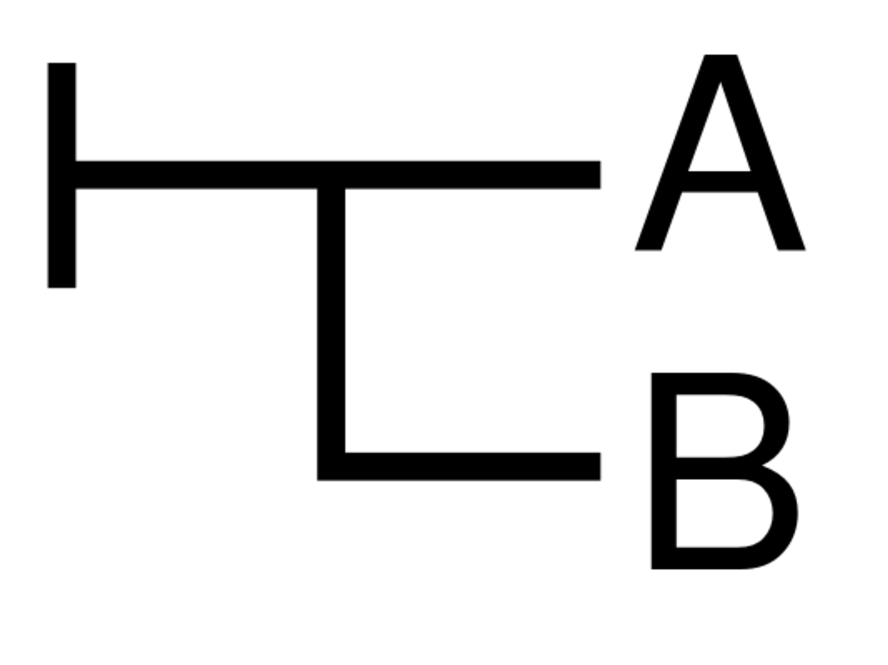
\includegraphics[height=1cm]{kondicionaliskis.eps}}
\item Modal / Temporal Logic (Saul Kripke: 1959)
\begin{itemize}
\item<4-> Modal: \emph{necessarily} true vs. \emph{possibly} true. 
\item<4-> Temporal: propositional logic plus \emph{always}, and \emph{eventually}
\item<5-> ``All men are dead.'' vs. ``\emph{Eventually}, all men are  dead.''
\end{itemize}
\end{itemize}
\end{wideslide}


\begin{wideslide}[bm=,toc=]{Important Features Across All Systems} 
%Logic PL FOL PTL/TPTL
%Truth static static dynamic
%Satisfiability static static dynamic
%Validity complexity
%Induction strong strong weak mutual
\begin{itemize}
\item Syntax
\begin{itemize}
\item<2-> Alphabet 
\item<2-> Formation rules
\end{itemize}
\item Semantics
\begin{itemize}
\item<3-> Interpretations
\item<3-> Truth (static or dynamic?)
\item<3-> Satisfiability
\item<3-> Validity
\end{itemize}
\item<4-> ``Mechanical support''---what can we automate?
\end{itemize}

\end{wideslide}


\begin{wideslide}[bm=,toc=]{Categories of logic}
The need for different forms of logic:
\begin{itemize}
\item Suppose $U$ is a universe of potential subscribers. 

\item Among them are paying {\em subscribers\/}
$s_1, s_2,\ldots$.

\item $\id{paids}_1,\id{paids}_2,\ldots$ 

\hspace{1em}subscribers represented by propositional variables

\hspace{1em}unwieldy for a large number of subscribers

\item $\forall s\in U.\,s\in \id{paid}$  
%\item $\forall s\in U.\,\id{paid}(s)$

\hspace{1em}subscribers represented by quantification over relation $\id{paid}$

\item $\forall s\in U.\,s\in \id{paid}(\bid{now})$

\hspace{1em}$\id{paid}$ relation is {\em dynamic\/} ($\bid{now}$ is current time)

A user is a subscriber if a fee has been paid in the last 6 weeks.

$\id{paid}(\bid{now}) = \{u\,|\,(u,t)\in \id{PaidWhen} \wedge \bid{now}-6 < t < \bid{now}\}$.

$s\in\id{paid}(t)$ may be true and $s\in\id{paid}(t+1)$ false.

\end{itemize}
\end{wideslide}

\end{document}
